\section{Problema C - Estimación mediante polinomios cúbicos}

Determine ahora una estimación de la edad de la muestra utilizando un polinomio de interpolación cúbico hacia adelante utilizando como punto de partida el dato correspondiente a i = 2. Presente también la expresión explícita del polinomio interpolador. Repita este apartado utilizando otro polinomio de interpolación cúbico hacia adelante con punto de partida i = 3. Utilice para ambos casos el método del interpolador de Lagrange.

\subsection{Resolución}

\subsubsection{Programación}

\paragraph{Generación de polinomios} Los polinomios de orden 3 se generan con el código descrito en \ref{gen_polynomials}:

\lstinputlisting[language=Python, firstline=47, lastline=64]{../../code/methods/lagrangian_interpolation.py}

Esto nos dará cinco polinomios, de los cuales solo usaremos dos, como en el siguiente snippet del código de los ejercicios.

\lstinputlisting[language=Python, firstline=16, lastline=16]{../../code/pecs/pec3/ex3.py}

\newpage 

\subsubsection{Polinomios generados vs muestras}

Una vez obtenidos los polinomios, pasamos a visualizarlos gráficamente.

\begin{figure}[H]
	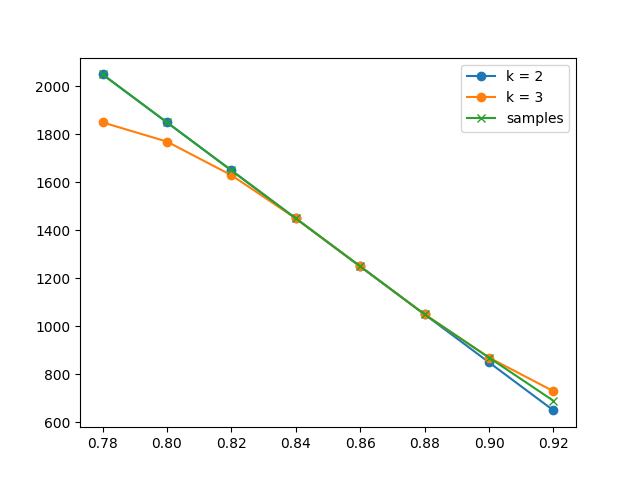
\includegraphics[width=\linewidth]{figures/figure2.png}
	\caption{Gráfica polinomios orden 3 y la muestra}
	\label{fig:interp_cub}
\end{figure}

Como es de esperar, vemos que los polinomios concuerdan más que nada en el rango que se usó para generar los polinomios (en especial a partir de k = 3).

\newpage 
\paragraph{} 
Esto queda ilustrado en la siguiente figura, donde vemos la diferencia entre los dos polinomios. 

\begin{figure}[H]
	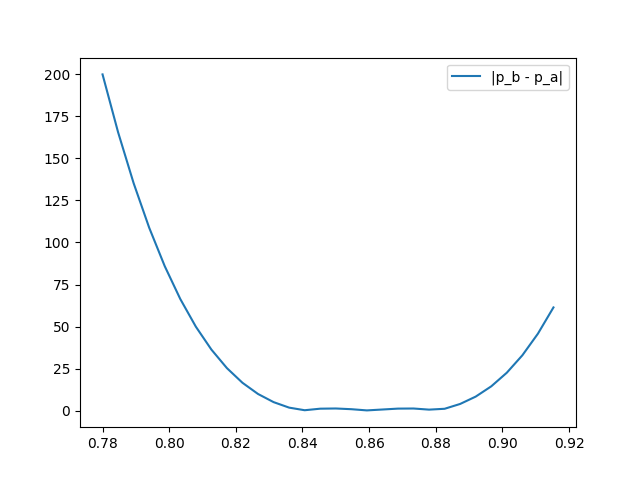
\includegraphics[width=\linewidth]{figures/figure3.png}
	\caption{Diferencia de los polinomios cúbicos}
	\label{fig:diff_interp_cub}
\end{figure}


\subsubsection{Resultados} 

Las edades interpoladas con los dos polinomios cúbicos ($k=2$, $k=3$) se ven en la siguiente tabla.

\begin{table}[htbp]
	\centering
	\csvreader[
	tabular=|c|c|c|,
	table head=\hline \textbf{\#} & \textbf{Age} \\\hline,
	late after last line=\\\hline,
	]{data/age02.csv}{}{\csvlinetotablerow}
\end{table}

